\documentclass[paper=a4, parskip=half]{scrreprt}

\usepackage{etex}
\usepackage[utf8]{inputenc}
\usepackage[T1]{fontenc}

\usepackage{lmodern}
\usepackage[ngerman]{babel}

\usepackage{bibgerm} 
\usepackage{cite}
\usepackage{url}

\usepackage{graphics}

\usepackage[hypertexnames=false, linktocpage]{hyperref}

\usepackage{titling}
\usepackage{graphicx}
\graphicspath{ {./Bilder/} }
\usepackage{wrapfig}
\usepackage{float}
\usepackage{adjustbox}
\usepackage{setspace}
\usepackage{hyperref}
\usepackage[acronym]{glossaries}
\usepackage{datetime}
\usepackage[normalem]{ulem}
\usepackage{color}

\usepackage{subfiles} % Best loaded last in the preamble

\subfile{Meta/glossary}

\setcounter{tocdepth}{1}

%Custom commands
\newcommand{\Genderly}{\textsc{Genderly }}

\begin{document}
%TC:ignore
\title{Politeia} % Meta

\subfile{Meta/coversheet}
\subfile{Meta/guides}


%Dieses Projekt ist Teil einer Studienarbeit der Hochschule für Wirtschaft und Recht Berlin. Das Projekt erzielt damit keine kommerzielle Absicht und dient als Lehrmethode für das Modul ''Software Engineering I''.
%Zu Beginn des Projekts gab es von den Betreuer*innen der Hochschule die Anforderung eines der 17 Sustainable Development Goals der United Nations \cite{UNGoals} zu erfüllen. Ebenso wurden Anforderungen zu Dokumentationsthemen und zeitliche Fristen gesetzt.


%TC:endignore
%Alternativ zu Geschäftlich würde auch Unternehmehrisch passen
\chapter{Problemstellung} \label{Problemstellung}
Im Rahmen des Moduls Software Engineering I des dritten Semesters im dualen Studium für Informatik wird von den Student*innen gefordert, in Gruppen ein Softwareprojekt zu planen, die Anforderungen an die Software zu erheben und einen Prototyp zu implementieren. \\
Noch vor der Idee für die Softwarelösung gab es von den Dozent*innen die Anforderung, eines der 17 Sustainable Development Goals der United Nations \cite{UNGoals} zu unterstützen. Ebenso wurden Anforderungen zu Dokumentationsthemen und zeitliche Fristen durch die Dozent*innen des Moduls gesetzt.

Dieses Softwareprojekt, welches den Namen \Genderly trägt, beschäftigt sich mit dem fünften Ziel, der Erreichung der Geschlechtergleichstellung. Dies wird im Folgenden genauer erläutert.

Das Gendern findet immer mehr Anwendung, insbesondere im pädagogischen, wie auch im akademischen Bereich. Unterschiedlichste Berufs- und Bildungsgruppen möchten inhaltlich saubere Arbeiten liefern und gleichzeitig einwandfrei und konsistent z.B. entweder mit Stern oder Doppelpunkt gendern. So werden unter anderem wissenschaftliche Arbeiten von Student*innen in genderneutraler Sprache verfasst, Artikel und Recherchen durch Journalist*innen werden genderneutral publiziert. \\
Das Schreiben von genderneutralen Texten wirkt für viele zu Beginn recht schwer. Es gibt viele neue Begrifflichkeiten und Möglichkeiten, wie gegendert werden kann. Es bedarf einer individuellen Eingewöhnungszeit. \\
\Genderly soll dahingehend viele Hürden nehmen. \Genderly soll ein System werden, in das Nutzer*innen Text eingeben können. Zum Text erstellt es einen genderneutralen Vorschlag. Verfasser*innen behalten ihren Fokus so weiterhin auf inhaltlicher Arbeit, die Aufgabe des Genderns wird abgenommen. \\
Damit der Aufwand für das Gendern der Texte erleichtert wird, muss die Software einfach und intuitiv bedienbar sein. Ein komplexes Softwareprodukt, welches schwer zu erlernen ist, würde den Zweck verfehlen, da in dem Falle der Aufwand für die Nutzer*innen an einer anderen Stelle aufkommt.


Zusätzliche Informationen lassen sich im \textit{Vision and Scope Dokument} sowie der \textit{Stakeholderanalyse} im \textcolor{blue}{\nameref{ch:Anhang}} finden.

\chapter{Problemlösung}

Die Software soll den Nutzer*innen helfen die anfänglichen Schwierigkeiten des Genderns zu überwinden. Dabei soll die Anwendung leicht und intuitiv bedienbar sein. Außerdem muss die Applikation für viele Personen nutzbar sein. \\
Aufgrund der benötigten Verfügbarkeit für die breite Masse ist \Genderly als Webanwendung ausgelegt. Die App kann dadurch möglichst einfach über eine Vielzahl unterschiedlicher Endgeräte erreicht und genutzt werden.

Das Layout von \Genderly{} orientiert sich grundlegend an dem Design eines Übersetzungsprogramms (siehe Abbildung \ref{fig:Screenshot}). Die App bietet den Nutzer*innen die Möglichkeit, den Eingabetext in einem Textfeld einzugeben und die Analyse des eingegebenen Texts und die Generierung des genderneutralen Alternativtexts mit einem Knopf zu starten. Außerdem bietet \Genderly ein weiteres Textfeld für die Textausgabe und Nachbearbeitung des Ausgabetextes. 
Durch die Ähnlichkeit zu einem Übersetzungsprogramm besitzt die Anwendung eine intuitive Bedienoberfläche und verfügt darüber hinaus auch über einen Wiedererkennungscharakter. Des Weiteren besteht die Weboberfläche aus wenig Elementen. Dies erhöht die Übersichtlichkeit der Anwendung.
Die Anwendung stellt auch ein Auswahlmenü für die Sprachauswahl (z.B. Deutsch, Englisch, etc.), den Gendering-Stil (z.B. Doppelpunkt-, Sternchen-Schreibweise, gänzlicher Wortersatz, etc.) und die Theme-Auswahl (heller oder dunkler Modus) bereit. Außerdem ist auf der Webseite ein Link zum GitHub Repository von \Genderly vorhanden, um die Transparenz zu erhöhen.


\begin{figure}[hbt!]
  \centering
  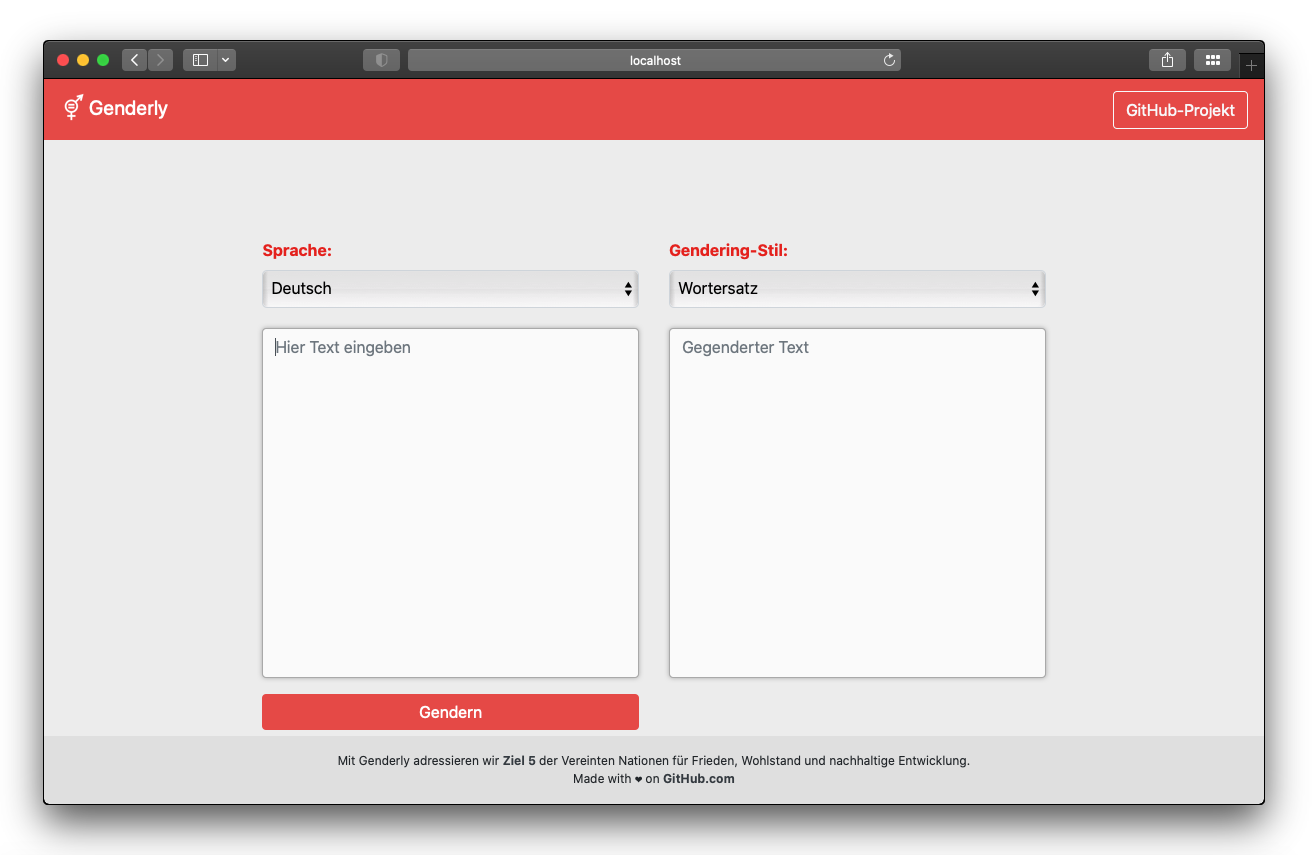
\includegraphics[scale=0.4]{Bilder/Genderly_Web.PNG}
  \vspace{-0.25cm}
  \caption[Screenshot der Webanwendung]{Screenshot der Webanwendung}
  \label{fig:Screenshot}
\end{figure}

Funktionsweise, Aufmachung und Gegenüberstellung machen \Genderly nicht nur zu einer Arbeitshilfe, sondern auch zu einem Lernmittel für korrektes Gendern.

In der Planungsphase wurden verschiedene Diagramme erstellt um einen reibungslosen Ablauf zu ermöglichen. Eines dieser Diagramme ist ein UML-Aktivitätsdiagramm, welches in Abbildung \ref{fig:Aktivitaetsdiagramm} zu sehen ist. Aktivitätsdiagramme werden verwendet, um Prozessabläufe darzustellen.

\begin{figure}[hbt!]
  \centering
  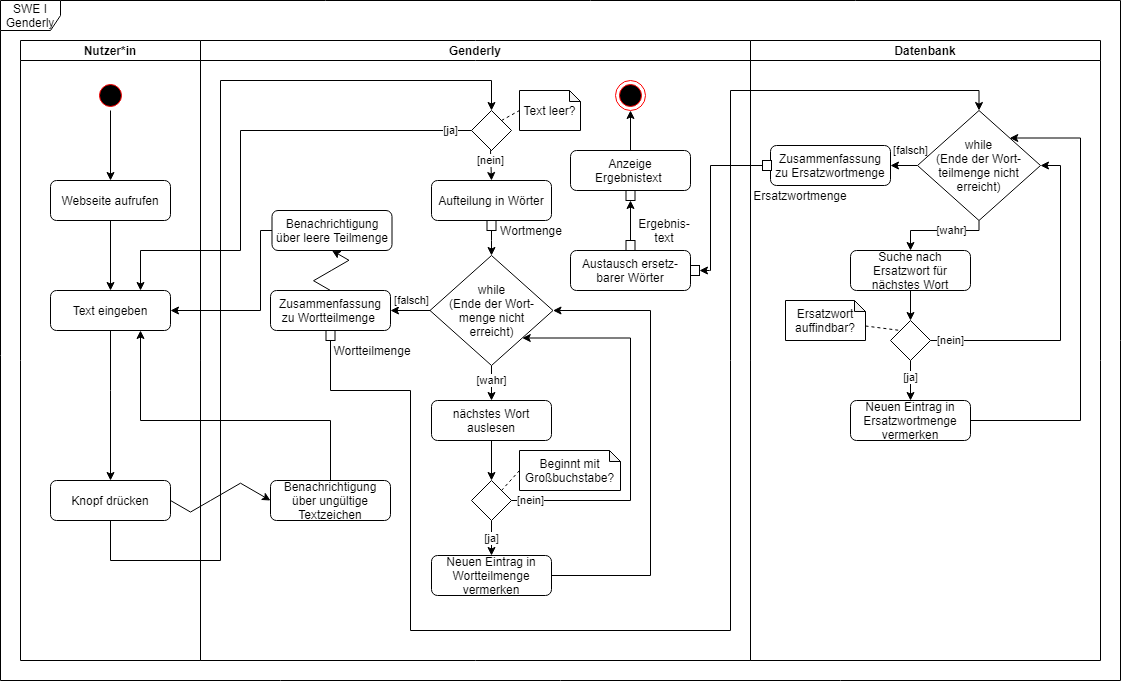
\includegraphics[scale=0.35]{Bilder/Aktivitaetsdiagramm.png}
  \vspace{-0.25cm}
  \caption[UML-Aktivitätsdiagramm für Genderly]{UML-Aktivitätsdiagramm für \Genderly}
  \label{fig:Aktivitaetsdiagramm}
\end{figure}

Der vorliegend mit dem Aktivitätsdiagramm beschriebene Prozess aus Textaufnahme, Verarbeitung und Ausgabe bildet die Kernkompetenz der Anwendung \Genderly. Bei \Genderly handelt es sich um eine Webanwendung. Der Prozess kann entsprechend während der Laufzeit beliebig oft wiederholt werden, da der Web-Server nach Prozessende weiterläuft.\\
Eine Interaktion beginnt mit dem Öffnen der Weboberfläche durch eine*n Nutzer*in, sowie die nutzer*innenseitige Texteingabe eines syntaktisch korrekten Texts. Sobald ein Knopf gedrückt wird, erfährt der Text eine Prüfung auf ungültige Zeichen, z.B. Steuerzeichen des ASCII-Zeichensatzes. Sollte Derartiges im Text gefunden werden, oder gar ein leerer Text vorliegen, wird der Nutzer bzw. die Nutzerin um wiederholte Eingabe gebeten.\\
Ein für gültig befundener, eingelesener Text wird in eine Menge aus Wörtern zerlegt. Von dieser Menge wird eine Teilmenge aus allen Wörtern gebildet, die mit einem Großbuchstaben beginnen. Diese Menge umfasst allgemein in deutschen Texten zwingend die Wortteilmenge der Substantive, enthält u.U. aber auch z.B. Artikel oder Wörter an Satzanfängen. Diese Teilmenge darf nicht leer sein, wenn es sich um geforderte, syntaktisch korrekte Texte handelt. Sollte sie leer sein, wird der Nutzer bzw. die Nutzerin erneut um Eingabe gebeten.\\
Die Wortteilmenge wird an eine Datenbank weitergeleitet. Sie versucht nun pro Wort eine Menge vermerkter Ersatzwörter zu finden. Diese Menge wird dem Ausgangswort zugewiesen. Wiederum diese Zuordnung von Wort zu Ersatzwortmenge wird einer globalen Ersatzwortmengen-Struktur hinzugefügt. Mit den Aufschlüssen aus dieser Struktur werden die ersetzbaren Wörter nun ersetzt. Sowohl Substantive als auch die mit ihnen assoziierten Artikel werden analysiert und ersetzt, damit der Ausgangstext grammatikalisch korrekt ist.  Der aus alten Satzteilen und Ersatzwörtern zusammengesetzte, neue Text wird abschließend angezeigt.

Die Struktur der Datenbank wird in der Abbildung \ref{fig:ERM} dargestellt.
ERM ist die Abkürzung für ``Entity Relationship Model''. Das ERM ist ein gängiger Modelltyp für die visuelle Repräsentation der Struktur einer Datenbank. 

\begin{figure}[hbt!]
  \centering
  \fbox{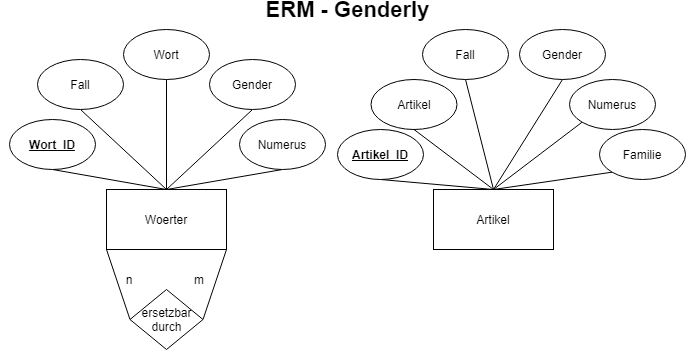
\includegraphics[scale=1.0]{Bilder/ERM.png}}
  \vspace{-0.25cm}
  \caption[ERM der Datenbank]{ERM der Datenbank}
  \label{fig:ERM}
\end{figure}

Das ERM erwartet eine bestimmte Vorgehensweise seitens des Programms.
Das Programm durchläuft den Eingabetext satzweise. Drei aufeinanderfolgende Wörter werden gleichzeitig betrachtet, dann wird um ein Wort weitergeschoben. \\
Sollte der gesamte Text eines Satzes unter drei Wörtern liegen, werden alle Wörter auf Einträge in der Tabelle ``Woerter'' untersucht. Gibt es von einem oder beiden Wörtern ein Substantiv bzw. einen ``Woerter-Eintrag'' wird ein Ersatzwort in ``Ersetzbarkeit'' gesucht. Wenn es kein Ersatzwort gibt, ist das Wort ordentlich gegendert, es bedarf keines Austauschs. Wenn es einen Eintrag gibt, wird überprüft, ob das Ersatzwort ein anderes Gender als das auszutauschende Wort besitzt. Wenn dies der Fall ist, wird das andere Wort aus dem Satz darauf überprüft, ob es sich um einen Artikel (``Der'', ``Die'', ``Das'', ``Ein'', ``Eine'') handelt und es wird mit einem Artikel derselben Artikelfamilie und dem passenden Fall (Kasus, Numerus, Genus) ersetzt. \\
Sollte ein Satz drei oder mehr Wörter besitzen, wird über den Satz iteriert. Es werden - wenn möglich - drei aufeinanderfolgende Wörter genommen, analysiert und ein Wort weitergegangen. Bei der Analyse ist das Mittelwort wichtig. Es wird überprüft, ob das Wort in ``Woerter'' vermerkt ist. Wenn es nicht vermerkt ist, dann wird ein Schritt bzw. ein Wort weitergegangen. Wenn es vermerkt ist, wird abgefragt ob es ersetzbar ist. Ist dem nicht so, dann ist das Wort gut gegendert. Wenn das jedoch der Fall ist, wird das Ersatzwort abgerufen. Jetzt wird wieder das Wort vor und nach dem Substantiv untersucht. Wenn die Wörter Einträge in der ``Artikel''-Tabelle haben, werden sie mit einem Artikel passend zum Fall und zum (Wort- nicht Bedeutungs-) Gender des Ersatzworts ersetzt.

Das Frontend, welches die Weboberfläche beinhaltet, ist mit HTML5, CSS3, JavaScript und Thymeleaf verfasst. Der Code für das Backend, welches mit dem Frontend und einer Datenbank kommuniziert, wurde mit Java unter Verwendung von Spring und Maven erstellt. Die Datenbank verwendet als Datenbankmanagementsystem SQLite.


Eine detailliertere Beschreibung der konkreten Ausgestaltung des aktuellen Prototyps und der folgenden Releases ist im \textit{Vision and Scope Dokument} und in der\textit{Software Requirements Specification} im \textcolor{blue}{\nameref{ch:Anhang}}.


\chapter{Ziele}
\section{Grundfunktionalitäten}
\label{sec:Grundfunktionalitäten}
Folgende Funktionalitäten der Anwendung sind geplant:

\begin{table}[!htb]
\begin{tabular}{ll}
\textbf{Funktionalität 1} & Aufrufbarkeit der Anwendung über eine eigene Weboberfläche. \vspace{0.1cm} \\
\textbf{Funktionalität 2} & Aufnahme von Text über eigenes Eingabefeld. \vspace{0.1cm} \\
\textbf{Funktionalität 3} & Auswahlmöglichkeiten für die Sprache des Texts. \vspace{0.1cm} \\
\textbf{Funktionalität 4} & Auswahlmöglichkeiten für den Gendering-Stil des durch eine \\
 & Analyse auszugebenden Text-Vorschlags. \vspace{0.1cm} \\
\textbf{Funktionalität 5} & Ermittlung und ggf. Austausch genderbarer Substantive. \vspace{0.1cm} \\
\textbf{Funktionalität 6} & Ermittlung und ggf. Austausch durch Gendering \\
& verfälschter Artikelzuordnungen. \vspace{0.1cm} \\
\textbf{Funktionalität 7} & Anpassung der farblichen Darstellung durch Nutzer*innen \vspace{0.1cm} \\
\textbf{Funktionalität 8} & Visualisierung des Ausgabetextes, sodass Nutzer*innen den \\
 & Ausgabetext noch nachbearbeiten können. \vspace{0.1cm} \\
\end{tabular}
\end{table}

\begin{figure}[hbt!]
  \centering
  \fbox{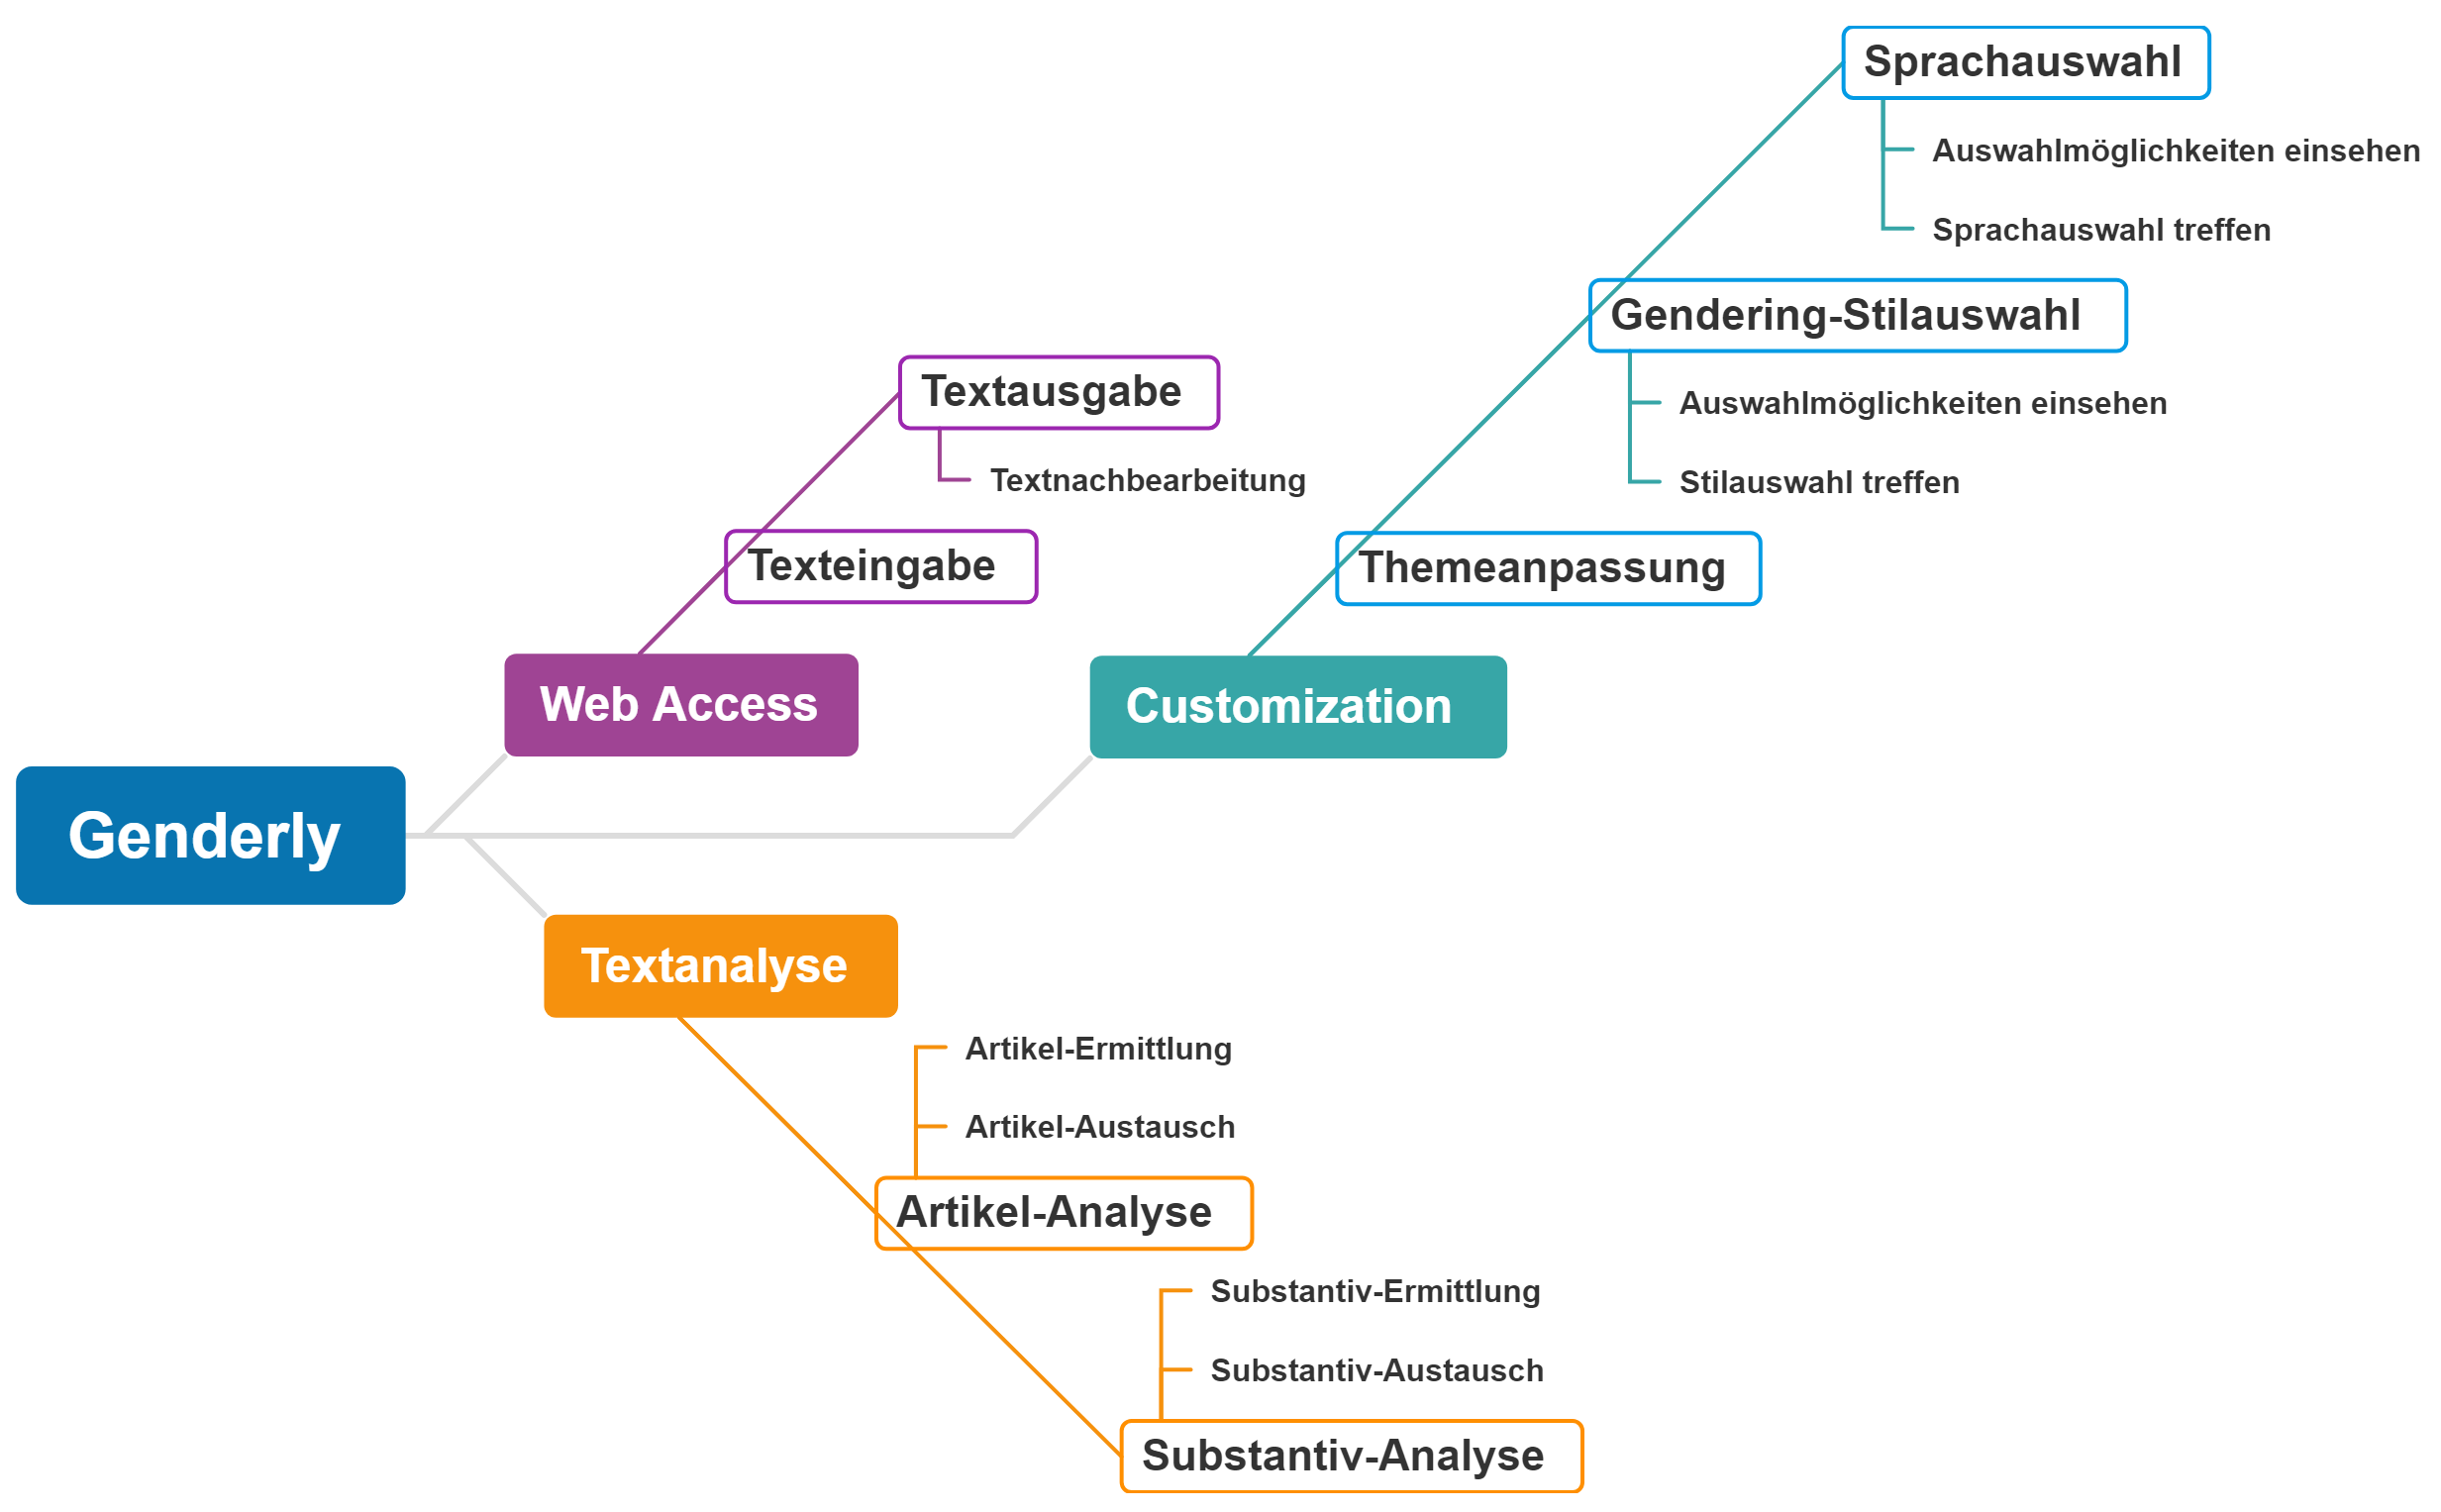
\includegraphics[scale=0.185]{Bilder/Genderly_FeatureTree.png}}
  \vspace{-0.25cm}
  \caption[Partieller Feature Tree]{Partieller Feature Tree}
  \label{fig:FeatureTree}
\end{figure}

Die erste Version besteht \textbf{nicht} aus einer vollständig realisierten und zu veröffentlichenden Anwendung. Sie stellt einen Prototyp für eine Teilmenge der unter \ref{sec:Grundfunktionalitäten}: \nameref{sec:Grundfunktionalitäten} aufgestellten Features dar, welche zwingend notwendig für die Funktionsfähigkeit der Anwendung sind (auch bekannt als Must-Haves). Im Folgenden ist die Auflistung dieser Funktionalitäten zu finden.

\begin{table}[!htb]
\begin{tabular}{ll}
\textbf{Funktionalität 1} & Aufrufbarkeit der Anwendung über eine eigene Weboberfläche. \vspace{0.1cm} \\
\textbf{Funktionalität 2} & Aufnahme von Text über eigenes Eingabefeld. \vspace{0.1cm} \\
\sout{\textbf{Funktionalität 3}} & \sout{Auswahlmöglichkeiten für die Sprache des Texts.} \vspace{0.1cm} \\
\sout{\textbf{Funktionalität 4}} & \sout{Auswahlmöglichkeiten für den Gendering-Stil des durch eine} \\
 & \sout{Analyse auszugebenden Text-Vorschlags.} \vspace{0.1cm} \\
\textbf{Funktionalität 5} & Ermittlung und ggf. Austausch genderbarer Substantive. \vspace{0.1cm} \\
\textbf{Funktionalität 6} & Ermittlung und ggf. Austausch durch Gendering \\
& verfälschter Artikelzuordnungen. \vspace{0.1cm} \\
\sout{\textbf{Funktionalität 7}} & \sout{Anpassung der farblichen Darstellung durch Nutzer*innen} \vspace{0.1cm} \\
\textbf{Funktionalität 8} & Visualisierung des Ausgabetextes, sodass Nutzer*innen den \\
 & Ausgabetext noch nachbearbeiten können. \vspace{0.1cm} \\
\end{tabular}
\end{table}

Nachträgliche Lieferungen sollen in erster Linie zur Komplettierung der verfügbaren Grundfunktionalitäten dienen (auch bekannt als Nice-To-Haves). Das Kernproblem, der Erstellungsgrund für \Genderly, wurde bereits mit dem Prototyp adressiert. Zukünftige Lieferungen können in noch nicht festgelegter Reihenfolge die hier aufgeführten Funktionalitäten beitragen:

\begin{table}[!htb]
\begin{tabular}{ll}
\textbf{Nachtrag 1} & Auswahlmöglichkeiten für die Sprache des Texts. \vspace{0.1cm} \\
\textbf{Nachtrag 2} & Auswahlmöglichkeiten für den Gendering-Stil des durch eine \\
 & Analyse auszugebenden Text-Vorschlags. \vspace{0.1cm} \\
\textbf{Nachtrag 3} & Anpassung der farblichen Darstellung durch Nutzer*innen \vspace{0.1cm} \\
\textbf{Nachtrag 4} & Präsenz von \Genderly auf Social Media herstellen \vspace{0.1cm} \\
\end{tabular}
\end{table}

In Absprache mit den Nutzer*innen werden diese möglichen Features je Release-Zyklus priorisiert implementiert oder gar verworfen.

\section{Personengruppen}
Da im akademischen Raum das Gendern deutlich und umfassend an Bedeutung gewinnt, ist entsprechend davon auszugehen, dass es sich bei den Nutzer*innen sehr wahrscheinlich zu einem großen Anteil um Student*innen handeln wird. Deshalb soll sich die Applikation auch genau an dieser speziellen Zielgruppe besonders orientieren. Die Anwendung soll den Student*innen beim einfachen und korrekten Gendern in wissenschaftlichen Texten helfen. Für Student*innen ist es wichtig, dass sie einen geringen Arbeitsaufwand haben, insofern muss die Anwendung einfach benutzbar sein.

\Genderly kann auch von Dozent*innen genutzt werden. Der Einsatz der Anwendung findet hier vorwiegend im didaktischen und pädagogischen Zusammenhang statt. Die Dozent*innen verfolgen dabei das Ziel ihren Lehrauftrag zu erfüllen, welcher auch die Vermittlung der Gleichberechtigung der Geschlechter beinhaltet. Dafür muss die Software einfache, flexible und mobile Anwendungsmöglichkeiten bieten. 

Eine weitere mögliche Nutzergruppe sind Lehrkräfte \& Schüler*innen. Die Lehrkräfte haben wie die Dozent*innen ein besonders hohes Interesse an der einfachen und flexiblen Anwendung des Produkts. Sie verfolgen ebenso das Ziel ihren Lehrauftrag zu erfüllen, welcher die Vermittlung der Gleichberechtigung der Geschlechter beinhaltet. Schüler*innen möchten gleichzeitig sehr leicht lernen. Beide nutzen die Software als Hilfsmittel während des Schreibens. Besonders hervorzuheben ist hierbei das potenzielle Alter der Anwender*innen sowohl in das eine, als auch in das andere Extrem. Die Software soll die Anwender*innen bei der Erweiterung ihrer Kenntnisse über genderneutrales Schreiben unterstützen. Aufgrund der großen Altersspanne ist eine stark vereinfachte Bedienung erforderlich.

Genauere Beschreibungen der Personengruppen und der Release-Planung lassen sich in der \textit{Stakeholderanalyse}, dem \textit{Vision and Scope Dokument} und in der \textit{Software Requirements Specification} im \textcolor{blue}{\nameref{ch:Anhang}} finden.


\chapter{Herangehensweise}

Dieses Kapitel befasst sich rein mit der Arbeit der Entwickler der Software gemeinsam als Team und mit der Herangehensweise innerhalb des Teams an das Projekt.

Das Thema Datenschutz wird sehr ernstgenommen und spielt international eine immer größer werdende Rolle worauf das Projektteam vorbereitet sein will. Deswegen ist die Entwicklung von \Genderly als Open-Source Projekt umgesetzt, sodass der Analyseprozess transparent gestaltet wird. \\
Das Projekt als solches wird dabei von den 4 Studenten angeleitet, deren Namen bzw. deren Benutzernamen sich einerseits auf dem Titelblatt befinden, andererseits auch in der offiziellen GitHub Organisation auffindbar sind.
Der gesamte Entwicklungsanteil steckt zu dem jetzigen Zeitpunkt zu 100\% bei genau diesen 4 genannten Studenten und es wurden keine weitere Einreichungen durch dritte zugelassen. Das ist wichtig anzumerken für die Bewertung und Einreichung der Software als Studienprojekt.

\Genderly ist als Open-Source Projekt auf der Plattform \href{https://github.com/HWR-Berlin-SWE-I-Gruppe-2-Team-3-2021/Genderly}{\textcolor{blue}{GitHub}} auffindbar.

Das 4-Personen-Team arbeitet in wöchentlichen Sprints in welchen die Studenten die aktuellen Entwicklungsfortschritte besprechen und somit alle Teammitglieder auf den neuesten Stand bringen, sowie das weitere Vorgehen planen. \\
Die gemeinsame Arbeit basiert auf dem sogenannten Vier-Augen-Prinzip. Das bedeutet, dass kein Mitglied die eigene Arbeit absegnet, sondern diese immer von einem weiteren Teammitglied geprüft und für gut befunden werden muss. Bei den Reviews wurden einige Fehler bereits durch GitHub Actions automatisiert geprüft, Syntaxfehler und nicht durchlaufende Unit-Tests konnten auf diese Weise keinen Weg in die fertige Softwarelösung finden. Alle Regeln des gemeinsamen Arbeitens sind zusätzlich schriftlich festgehalten in dem öffentlich einsehbaren Code of Conduct und den Contribution Guidelines des Projekts. \\
Ebenso wird das Thema Cyber-Security sehr ernst genommen, weshalb sich außerdem noch eine Security Policy im Projekt befindet. \\
Eigenständig erstellte Vorlagen auf GitHub helfen, den Fokus innerhalb der Entwicklung von repetitiven Aufgaben abzulenken. Die Entwicklung von \Genderly in einer GitHub-Organisation hilft bei der Organisation der verschiedenen Unterprojekte, welche sich während des Entwicklungszeitraums ergeben. So gibt es ein abgesondertes Projekt, in welchem sämtliche Dokumentationen und Präsentationen als Gruppe entwickelt und gespeichert werden.

Es ist geplant, dass die Entwicklung im weiteren Verlauf des Studiums der vier Teammitglieder weiter fortgesetzt wird und ggf. nach Abschluss des Studiums Beiträge Dritter zugelassen werden. \\
Das Softwareprojekt wird mit der MIT-Lizenz für alle Personen zur Verfügung gestellt, welche an der Entwicklung interessiert sind.
\Genderly verfolgt dabei keine monetären Aspekte. 

Das Softwareprojekt ist ein erster Linie ein Studienprojekt. Eine der Aufgaben war, dieses Projekt in einer sogenannten Zwischen- und Endpräsentation den Kommiliton*innen und Dozent*innen vorzustellen. Der Anlass wurde von uns, der Entwicklergruppe, genutzt, um Feedback einzuholen und Fragen zu beantworten. Die entstandenen Fragen bezogen sich zum Großteil darauf, wie ein syntaktisch und grammatikalisch korrekter Satz generiert wird, welcher seine Aussage nach Möglichkeit nicht verliert, abgesehen von der Änderung des Geschlechts der Substantive.

Die Funktionsweise von \Genderly{} wurde im vorherigen Kapitel behandelt. Jetzt folgen die Komplikationen, welche es in der Entwicklung gab.


\chapter{Komplikationen}
Bei der Planung und der Entwicklung der Software sind einige Komplikationen aufgetreten.
Das erste Problem wurde schon am Anfang der Planungsphase ersichtlich. Es musste zuerst beschlossen werden, wie die Analyse des Eingabetexts und die Generierung des genderneutralen Ausgabetexts umgesetzt werden sollte. Die beste Lösung dafür wäre eine KI (künstliche Intelligenz) zu erstellen und zu trainieren, damit die KI selbstständig die genderbaren Wörter aus dem Text raussucht, ersetzt und einen grammatikalisch korrekten und genderneutralen Text generiert. Auf diesem Prinzip beruhen auch die modernen Übersetzungsprogramme. Aufgrund des begrenzten Zeitrahmens wurde sich stattdessen für eine statische maschinelle Übersetzungsmethode entschieden, welche mit einer Datenbank arbeitet. Auf diese Art und Weise arbeitete auch der Google-Übersetzer in seinen frühen Jahren. \\
Das zweite Problem trat gleich auf, nachdem beschlossen wurde eine Datenbank zu verwenden und die Wörter statisch zu gendern. Es  stellte sich die Frage, wie die Textanalyse konkret gestaltet wird. Die erste Idee war, dass nur die genderbaren Wörter ersetzt werden, dies garantiert jedoch keineswegs für die grammatikalische Korrektheit des Ausgabetexts. Für die Lösung dieses Problems war eine tiefergehendere Recherche über die deutsche Grammatik vonnöten. Das Ergebnis ist, dass die genderbaren Wörter auf zugehörige Artikel und deren Fall (Kasus, Numerus und Genus) und Wort-Gender geprüft werden und diese entsprechend mit ausgetauscht werden. \\
Die Strukturierung der Datenbank bereitete auch Schwierigkeiten. Die Anzahl der Tabellen sowie deren Aufbau und die Beziehungen zwischen den Einträgen innerhalb der Tabellen waren zu Beginn noch unklar. Die endgültige Struktur der Datenbank ist in der Abbildung \ref{fig:ERM} dargestellt. \\
Das letzte Problem besteht immer noch. Die Datenbank muss mit den entsprechenden Wortlisten befüllt werden, was einen gewaltigen Zeitaufwand darstellt. Es gibt in der deutschen Sprache immens viele Substantive, welche auf genderneutrale Alternativen geprüft und in die Datenbank eingetragen werden müssen.


\chapter{Fazit und Ausblick}
Momentan ist der Prototyp der Software implementiert. Dies bedeutet, dass eine funktionsfähige Software vorhanden ist. Das Frontend bzw. die Weboberfläche, welche das Ein- und Ausgabefeld für den Text und die Verlinkungen auf das GitHub-Repository und auf die Webseite der 17 Sustainable Development Goals der United Nations beinhaltet, ist vollständig implementiert. Im Backend sind die Textanalyse und -bearbeitung sowie die Generierung des genderneutralen Ausgabetexts funktionsfähig, der Aufbau und die Einbindung der Datenbank sind auch vorhanden. Außerdem ist auch eine Art Immunsystem der Software implementiert, welches SQL-Injection-Attacken erkennt und verhindert. Bei SQL-Injection nutzen Cyberkriminelle gezielt Sicherheitslücken in der Software aus um unbefugt auf die Datenbank zugreifen und die verändern zu können. Dies wird bei \Genderly verhindert. Des Weiteren wurden mehrere Unit-Tests erstellt, welche die korrekte Funktionsweise der Software und ihrer Komponenten automatisch überprüft. \\
Die Datenbank noch nicht vollständig, sie beinhaltet einige Beispieldatensätze, welche verwendet wurden um die Funktionsweise der Anwendung zu überprüfen.
Damit ist eine prototypische Funktionalität der Software sichergestellt. Dazu entstanden während der Projektphase mehrere UML-Diagramme und Dokumente zur Anforderungsspezifikation für den Release 1.0, welcher der aktuelle Release ist. \\
Das Projekt ist öffentlich bei der GitHub-Organisation einsehbar. Dort ist es als Public Foss Projekt aufrufbar und umfasst u.a. Contribution Guidelines, einen Code of Conduct, eine Security Policy, eine Projektlizenz und vieles mehr.

Es ist ein lauffähiger Zwischenstand vorhanden, der alle Aspekte der Problemstellung adressiert, der technisch aber durchaus noch weiterentwickelt werden kann und auch wird.

Der Ausbau der Datenbank kann noch weiter verfolgt werden, sodass mehr Wörter erkannt und ausgetauscht werden können. 
Außerdem ist die Anwendungsarchitektur auf die Implementation der "Nice-To-Haves" vorbereitet, sodass \Genderly mit der Auswahl von verschiedenen Gendering-Stilen und Sprachen erweitert werden kann. \\
Der Projektmanagement-Aspekt ist auch nicht zu vernachlässigen. Die fortlaufende Aktualisierung der Vision und Strategie sowie der kontinuierliche Vergleich zwischen Ist- und Soll-Stand sind wichtige Aspekte. Außerdem sind weitere Interviews mit den Nutzer*innen möglich, damit \Genderly sich mithilfe deren Feedback stetig verbessert.

Für die Installationsanweisung der aktuellen Version klicken sie \href{https://github.com/HWR-Berlin-SWE-I-Gruppe-2-Team-3-2021/Genderly}{\textcolor{blue}{hier}}

Zusätzliche Informationen über den aktuellen Release und folgende Releases finden sie im \textit{Vision and Scope Dokument} und in der \textit{Software Requirements Specification} im \textcolor{blue}{\nameref{ch:Anhang}}.


%TC:ignore
%Glossar
\printglossary
\pagebreak

\nocite{*}
\bibliography{Literatur}
\bibliographystyle{alphadin}


\subfile{Anhang/main}
%TC:endignore

\end{document}